\chapter{Literature Study} 
\label{chap:2}
\section{Background}

\subsection{What is cross-ledger?}
\noindent Since the development of blockchain technology, many different chains have been born, and the information isolation of many chains inevitably forms the value island effect of blockchain. There is a need for a technology that can work with different blockchains and become the bridge connecting them. \\
\noindent Cross-ledger (or cross-chain) in the narrow sense is the process of asset/data interoperability between two relative independent blockchains.\\
\noindent Traditional ICT field defines the \textit{interoperability} as the ability to share and utilize information between different ICT systems or modules in a reliable way\cite{osello2015bim}. While \textsc{Vitalik Buterin} mentioned in \textsc{Chain Interoperability}\cite{buterin2016chain} that interoperability in the blockchain area mainly describes the ability of assets exchange, information intercommunication and atomic transactions between various blockchains. This can be achieved by introducing the third party without modifying the original chains.
\subsection{Evolution of Cross-chain}
\noindent As shown in Figure \ref{fig:his}, it has not been a short period for Ripple to release the \textit{Interledger Protocol}(ILP)\cite{thomas2015protocol} in 2012 since the advent of Bitcoin Network in 2009. Interledger protocol proposed a cross-ledger interoperability scheme for the first time in the blockchain area, which enables cross-ledger transfers through third-party notaries. In 2014, the BlockStream team, founded by the Bitcoin core developer group, first proposed a \textit{Pegged Sidechains} cross-chain interaction scheme, introducing a sidechain with a two-way peg to achieve cross- chain asset transfer. Soon in 2015, the Bitcoin Lightning Network\cite{poon2016bitcoin} adopted a \textit{Hashed Timelock} mechanism to implement a fast transaction channel off the Bitcoin main chain. In 2016, the BTC-Relay\cite{btc-relay} solution was released, and the one-way cross-chain communication from Bitcoin to Ethereum was realized based on the relay cross-chain scheme. In the same year, \textsc{Chain Interoperability}\cite{buterin2016chain} by Vitalik Buterin made a comprehensive and in-depth analysis of blockchain interoperability issues. In 2017, Polkadot and Cosmos first proposed a solution for building a cross-chain network infrastructure platform. Now the Cosmos hub blockchain has launched in March 2019.

    \begin{figure}[H]
    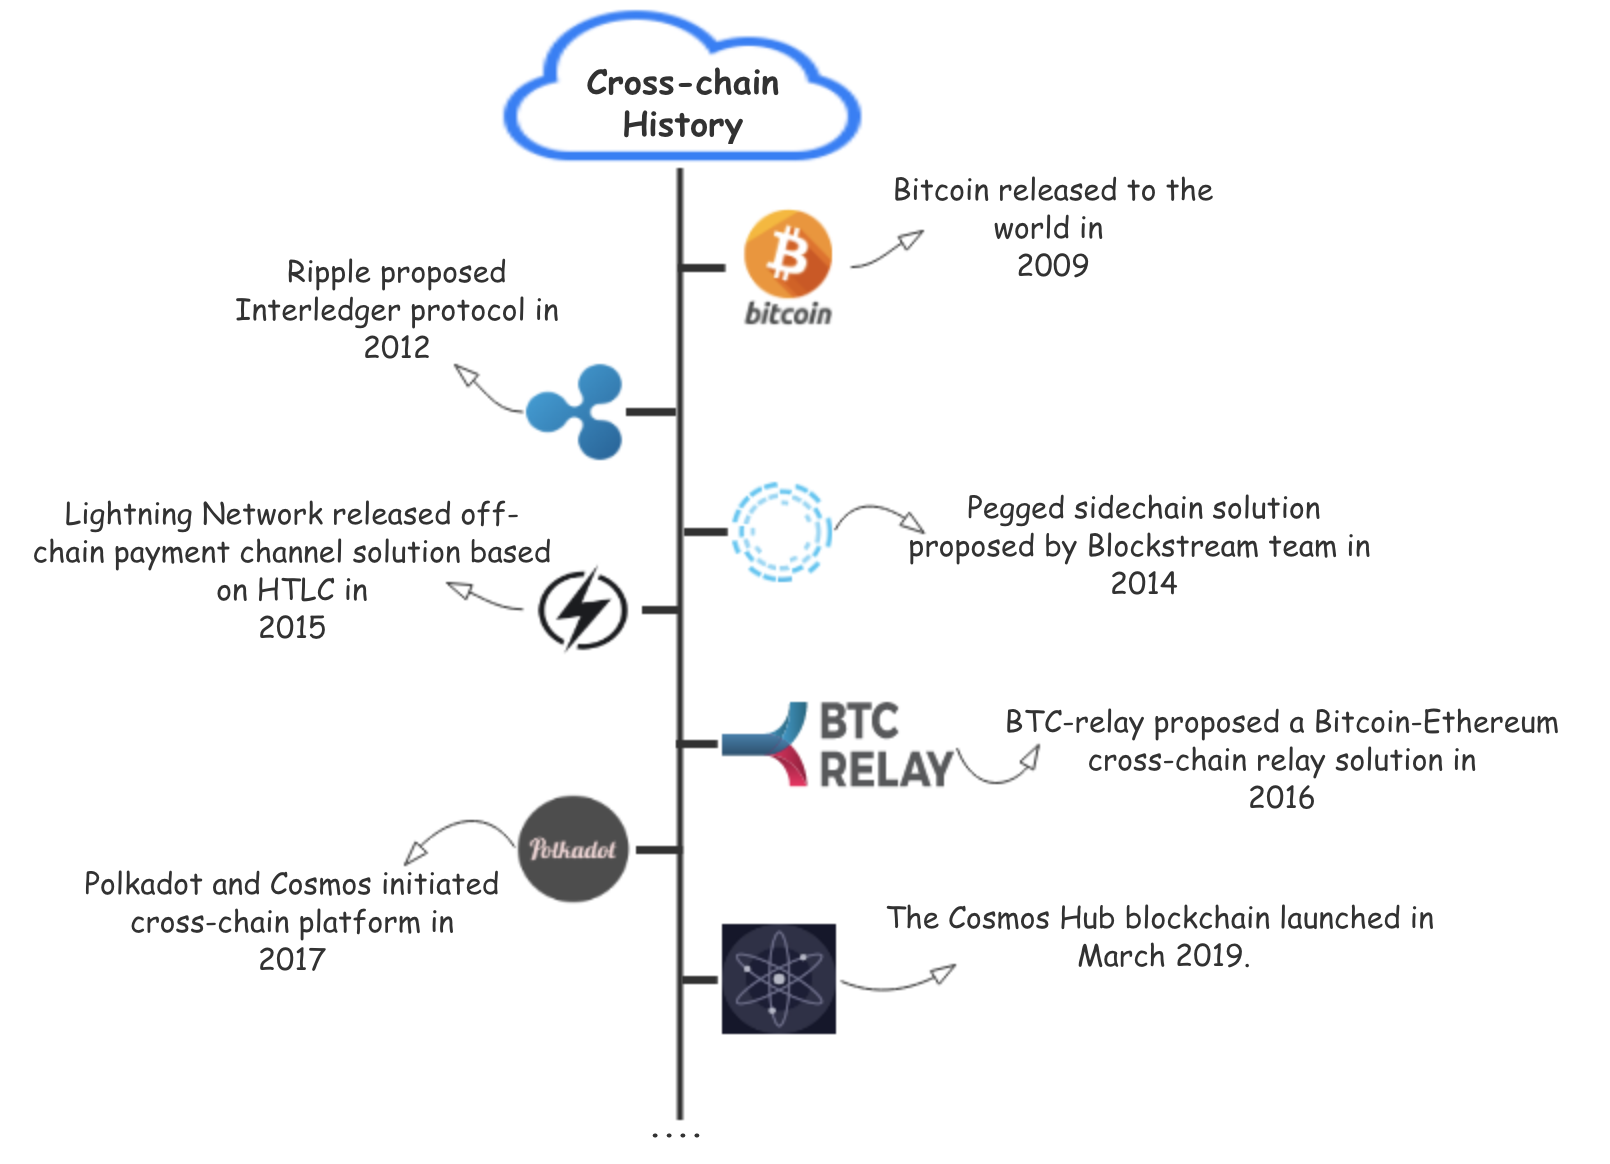
\includegraphics[width=1\textwidth]{./figures/his.png}
    \centering
    \caption{Cross-chain development tree}%\protect\footnotemark}
    \centering
    \label{fig:his}
    \end{figure}
    
\section{Cross-chain manifestation}
\noindent So far we know, current public blockchain is a self-adaptive, relatively closed distributed system. Although the system allows new nodes to join and old nodes exit, it also has its own fault-tolerant mechanism. It is hard to be compatible with external systems. \\
\noindent In a way, there are two main value/data interoperability implementations between chains:
\begin{enumerate}
    \item \textbf{Inter-chain asset exchange}: \\
    It usually refers to asset swapping between different users on both chains. However, the total amount of assets in each chain does not increase or decrease, instead, the ownership of the assets has changed. The process of this change needs to occur synchronously on both chains. \\
    \begin{figure}[H]
    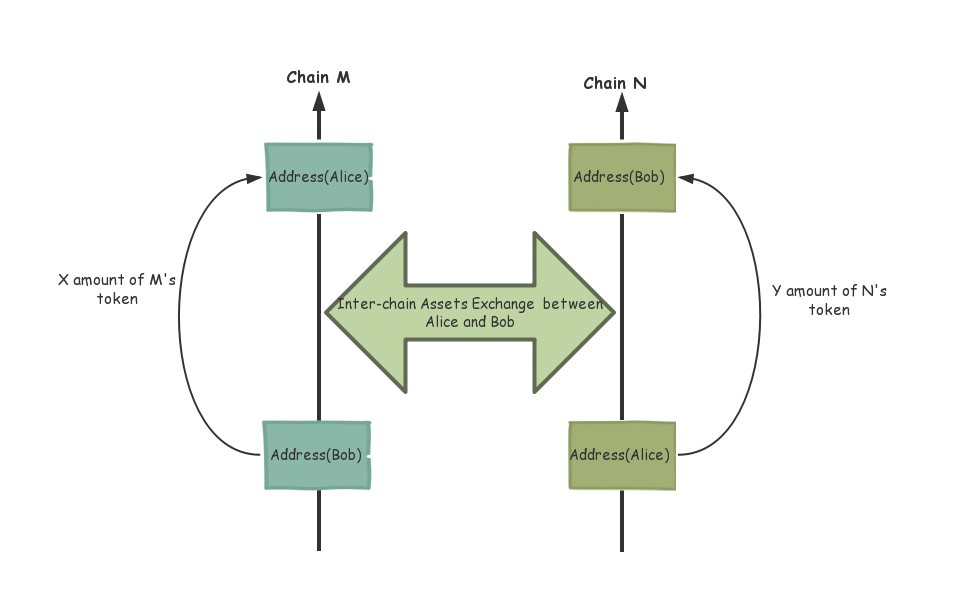
\includegraphics[width=1\textwidth]{./figures/asset_swap.png}
    \centering
    \caption{Inter-chain exchange diagram}%\protect\footnotemark}
    \centering
    \label{fig:swap}
    \end{figure}
    This diagram briefly describes the situation when Alice wants to use X amount of chain M's token exchange for Bob's Y amount of chain N's token. Eventually, Bob's token in chain N swaps to Alice's address in chain N, similarly, Alice's token swaps to Bob's address located in chain M.
    \item \textbf{Inter-chain asset transfer (one/two-way)}: \\
    Compared with the consistency in the total number of assets in the asset exchange, the transfer has a transfer of asset value, which is manifested in the increase or decrease of the available assets in each chain. For example in Figure \ref{fig:transfer}, the scenario is Alice wants to transfer X number of chain M's token to chain N, as a result, chain M send X amount of token to a locked address in original chain, in turn, chain N generates an equal amount of tokens of itself in a certain address that can be used. Thus, the transfer of this asset succeed.
    
    \begin{figure}[H]
    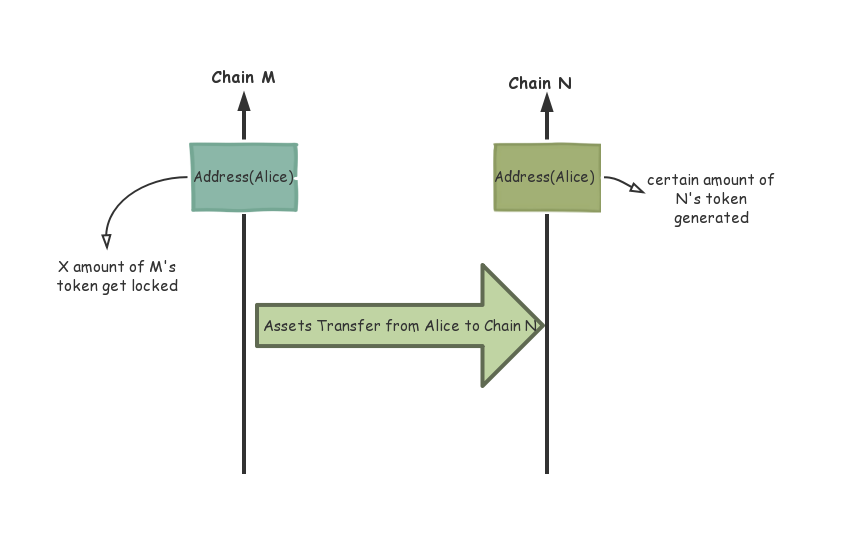
\includegraphics[width=1\textwidth]{./figures/transfer.png}
    \centering
    \caption{Inter-chain transfer diagram}%\protect\footnotemark}
    \centering
    \label{fig:transfer}
    \end{figure}
\end{enumerate}

\noindent For now, researches and applications of cross-chain are mainly focused on these two methods. Some projects have proposed the concept of cross-chain smart contracts, which is similar to the realization of cross-chain asset transfer in terms of technical implementation.

\section{Difficulties}
\noindent The number one feature in the blockchain is immutability, every record must be accurate to protect value. Hence, in the cross-chain project, the key point is to ensure the accuracy of each transaction. There are many obstacles cross-chain need to encounter. To sum up, the following are several key points:

\begin{itemize}
    \item \textbf{How to ensure the atomic of transactions.}\\
    That is, cross-chain transactions either occur or do not occur. Otherwise the inconsistency and "out-of-sync" status of the two chains will become the biggest system vulnerabilities in cross-chain transactions, and the security of both systems will be threatened. This is the basic requirement for realizing cross-chain transactions, and it is also a difficult point that must be solved in cross-chain transactions.
    \item \textbf{How to complete the confirmation of the transaction for other chains.} \\
    The confirmation including the transaction has occurred and is wound up and written into the right block as well as the transaction has been confirmed by enough blocks in the whole system so the probability of invalidation of the transaction due to system reconfiguration will be very low. Blockchains are lack of a mechanism to actively obtain external information, so it is not an easy task to confirm the trading status of another chain.
    \item \textbf{How to ensure that the total assets of the two chains remain unchanged.} \\
    In the scenario of asset exchange, the assets of the two chains are not substantially exchanged, so this type of situation does not change the total assets of each chain. However, in the scenario of asset transfer, the number of available assets in each chain changes, total assets can remain unchanged only when the cross-chain transactions are accurately recorded, and the accounting of the two chains is completely atomic, either at the same time or not. 
    \item \textbf{How to ensure the independent security of the two chains.} \\
    When two chains inter-operate, it is inevitable that they will affect each other. How to ensure the security of their own chains and the others in the process of cross-chain transactions is a problem worth considering. If the security issue cannot be isolated, then one attacked chain will affect the entire cross-chain network.
    \item \textbf{How to realize multiple chains interoperability.} \\
    Take the history of the computer network as a reference, the independent blockchain network will eventually embark on the future of interconnection. How to link these existing and future blockchain networks to be unified into one whole network will be one of the most important issues of the future cross-chain network. 
\end{itemize}


\section{Summary}

\noindent This chapter introduces a thorough background study of the cross-chain research area. It briefly reviews the history of cross-chain development and outlines the importance of the growing technology of cross-chain. Two main manifestations of cross-chain transactions are proposed to give a classification standard for Chapter \ref{chap:3} project study. Chapter \ref{chap:2} also describes the key difficulties that cross-chain projects facing. Some of them will be discussed in the following chapter.